\documentclass{TIJMUjiaoanLL}
\pagestyle{empty}


\begin{document}


%课程名称
\kecheng{Linux系统概论}
%课程内容
\neirong{高级Linux命令\ /\ 第8\&9章}
%教师姓名
\jiaoshi{伊现富}
%职称
\zhicheng{讲师}
%教学日期(格式:XXXX年XX月XX日XX时-XX时)
\riqi{2019年5月28日13:30-15:10}
%授课对象(格式:XXX系XXXX年级XX班(硕/本/专科))
\duixiang{生物医学工程与技术学院2017级生信班(本)}
%听课人数
\renshu{28}
%授课方式
\fangshi{理论讲授}
%学时数
\xueshi{2}
%教材版本
\jiaocai{Unix入门经典,第1版}


%教案首页
\firstHeader
\maketitle
\thispagestyle{empty}

\mudi{
\begin{itemize}
  \item 掌握常见的元字符,find的使用,grep的使用,sed的使用,AWK的使用。
  \item 熟悉正则表达式的构建,find的常用测试,grep的常用选项,sed的工作原理,AWK的工作原理和脚本结构。
  \item 了解Linux中的文本处理命令。
  \item 自学文本处理命令在生物信息学中的应用。
\end{itemize}
}

\fenpei{
\begin{itemize}
  \item (5')引言与导入:回顾Linux命令的基本格式以及常用的Linux命令,引申出授课内容。
  \item (20')正则表达式和元字符:介绍正则表达式和元字符的概念,讲解元字符中的字符、字符集、量词和边界,举例说明正则表达式的构建。
  \item (20')find和grep:讲解find的常用测试并通过实例进行演示,讲解grep的常用选项并通过实例进行演示。
  \item (5')文本处理命令:总结Linux中常用的文本处理命令。
  \item (40')sed和AWK:讲解sed的工作原理、定位规则和常用命令,通过实例演示sed的使用;讲解AWK的工作原理和脚本结构,通过实例演示AWK的使用。
  \item (5')生物信息学中的应用:举例说明文本处理命令在生物信息学中的应用。
  \item (5')总结与答疑:总结授课内容中的知识点与技能,解答学生疑问。
\end{itemize}
}

\zhongdian{
\begin{itemize}
  \item 重点:元字符,find的使用,grep的使用。
  \item 难点:元字符,sed的使用,AWK的使用。
  \item 解决策略:通过实例讲解与操作演示帮助学生理解、记忆。
\end{itemize}
}

\waiyu{
  \vspace*{-10pt}
  \begin{multicols}{2}
    正则表达式(regular expression)

    元字符(metacharacter)

    字符集(character class)

    模式空间(pattern space)
  \end{multicols}
  \vspace*{-10pt}
}

\fuzhu{
\begin{itemize}
  \item 多媒体:元字符,find的测试,grep的选项,sed和AWK的工作原理。
  \item 板书:常见的元字符,正则表达式的构建与解析。
  \item 演示:find、grep、sed和AWK的基本使用。
\end{itemize}
}

\sikao{
  \vspace*{-10pt}
  \begin{multicols}{2}
  \begin{itemize}
    \item 列举五个常见的元字符并解释其含义。
    \item 根据要求编写正则表达式。
    \item 根据要求使用find查找文件。
    \item 根据要求使用grep查找字符串。
    \item 根据要求组合使用文本处理命令。
    \item 根据要求编写sed脚本编辑文件。
    \item 根据要求编写AWK脚本输出特定字段。
    \item 根据要求处理生物信息学文本数据。
  \end{itemize}
  \end{multicols}
  \vspace*{-10pt}
}

\cankao{
\begin{itemize}
  %\item (美)Paul Love,Joe Merlino\ 等著,张楚雄,许文昭\ 译。Unix入门经典,清华大学出版社,2006。
  \item (美)Harley Hahn\ 著,张杰良\ 译。Unix \& Linux大学教程,清华大学出版社,2010。
  \item 鸟哥\ 著,王世江\ 改编。鸟哥的Linux私房菜——基础学习篇(第三版),人民邮电出版社,2010。
  \item (美)Ben Forta\ 著,杨涛\ 等译。正则表达式必知必会,人民邮电出版社,2007。
  \item 维基百科等网络资源。
\end{itemize}
}

\firstTail


%教案续页
\newpage
\otherHeader

\begin{enumerate}
  \item 引言与导入(5分钟)
    \begin{enumerate}
      \item 回顾:Linux命令的基本格式,常用的Linux命令
      \item 介绍:正则表达式和元字符,find、grep、sed、AWK等高级命令
    \end{enumerate}

  \item 正则表达式和元字符(20分钟)
    \begin{enumerate}
      \item 简介
	\begin{itemize}
	  \item 正则表达式:具有一定句法的集合或短语,包含元字符或普通字符,表示某类文本或字符串。
	  \item 元字符:代表一组字符或命令的字符,用最小的字符集表示多组文本。
	  \item 相关命令:less,more,grep,sed,AWK,vim,……
	\end{itemize}
      \item \textcolor{red}{\textbf{【重点、难点】}}元字符\textcolor{red}{(结合实例讲解每一个元字符)}
	\begin{itemize}
	  \item 字符:一般字符,\verb|.|,\verb|[]|,\verb|[a-z]|,\verb|[0-9]|,\verb|[^]|,\verb|\|
	  \item 字符集:\verb|\d|,\verb|\D|,\verb|\s|,\verb|\S|,\verb|w|,\verb|\W|
	  \item 量词:\verb|?|,\verb|*|,\verb|+|,\verb|{m}|,\verb|{m,n}|
	  \item 边界:\verb|^|,\verb|$|
	  \item 其他:\verb|()|,\verb=|=
	\end{itemize}
	\vspace*{-10pt}
	\begin{figure}[h]
	  \centering
	  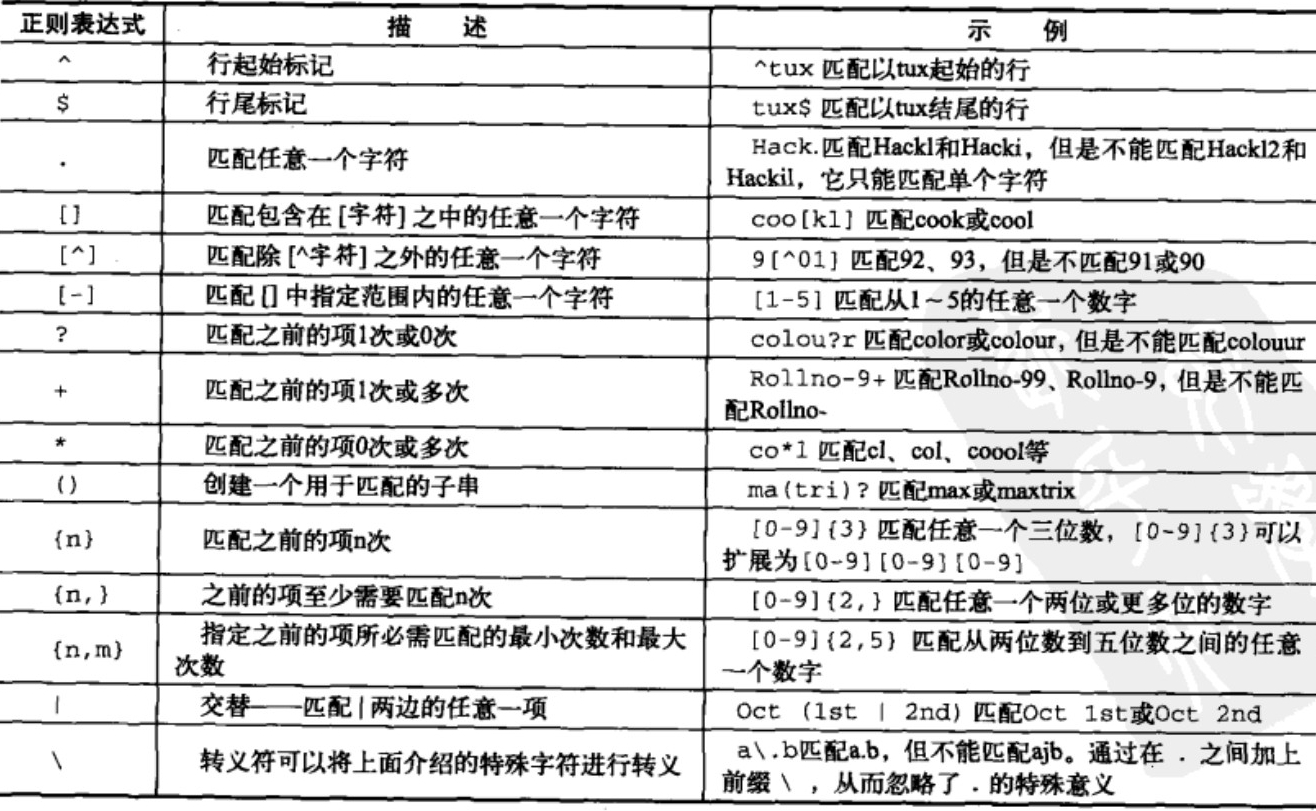
\includegraphics[width=15.5cm]{c5_meta_03.jpg}
	\end{figure}
	\vspace*{-10pt}
      \item 正则表达式
	\vspace*{-10pt}
	\begin{figure}[h]
	  \centering
	  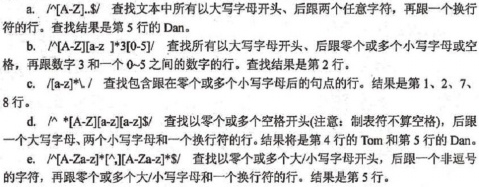
\includegraphics[width=15.5cm]{c5_re_example_02.jpg}
	\end{figure}
	\vspace*{-10pt}
    \end{enumerate}


\otherTail
\newpage
\otherHeader


  \item grep和find(20分钟)
    \begin{enumerate}
      \item \textcolor{red}{【重点】}find\textcolor{red}{(实例讲解、操作演示)}
	\begin{enumerate}
	  \item 测试
	\vspace*{-10pt}
	\begin{figure}[h]
	  \centering
	  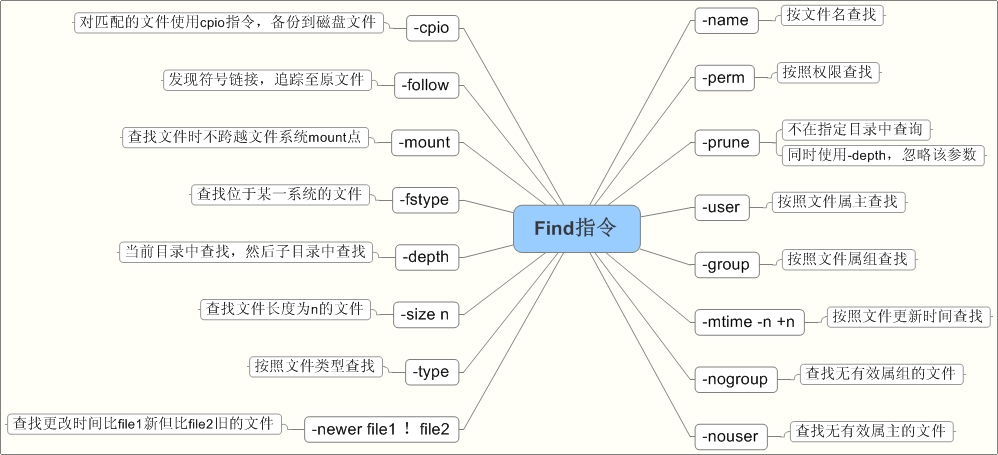
\includegraphics[width=15cm]{c5_find_01.jpg}
	\end{figure}
	\vspace*{-10pt}
	  \item 实例
	    \begin{itemize}
\parpic[fr]{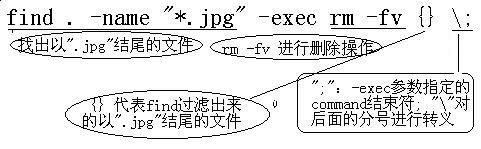
\includegraphics[width=8cm]{c5_find_02.jpg}}
	      \item \verb|find /etc -name passwd|
	      \item \verb|find /home -user USER|
	      \item \verb|find /home -size +2G -print|
	    \end{itemize}
	\end{enumerate}
      \item \textcolor{red}{【重点】}grep\textcolor{red}{(实例讲解、操作演示)}
	\begin{enumerate}
	  \item 简介
	  \begin{description}
	    \item[定义] Globally search a Regular Expression and Print(全局正则表达式打印)
            \item[功能] 在文件中搜索用户所指定的序列,然后将结果打印出来
            \item[用途] 搜索文件或者在文件中进行查找
            \item[结构] \verb|grep StringToSearchFor FileToSearch|
          \end{description}
	  \item 选项
	\vspace*{-10pt}
	\begin{figure}[h]
	  \centering
	  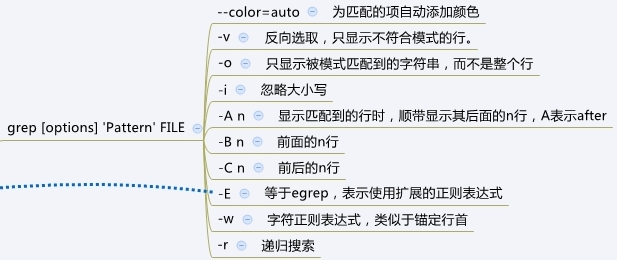
\includegraphics[width=14cm,height=5cm]{c5_grep_01.jpg}
	\end{figure}
	\vspace*{-10pt}
	  \item 实例
	\vspace*{-10pt}
	\begin{figure}[h]
	  \centering
	  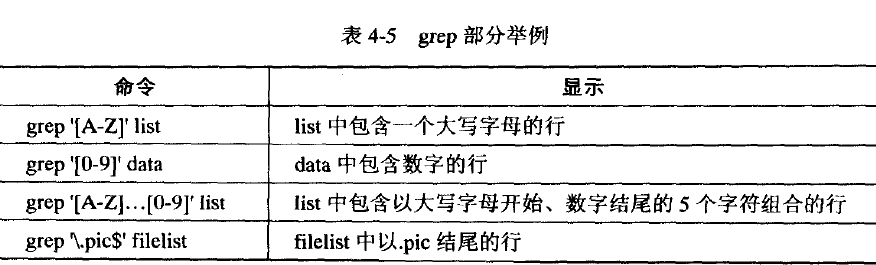
\includegraphics[width=14cm,height=3cm]{c5_grep_02.png}
	\end{figure}
	\vspace*{-10pt}
	\end{enumerate}
    \end{enumerate}

\otherTail
\newpage
\otherHeader


  \item 文本处理命令(5分钟)
	\vspace*{-10pt}
	\begin{figure}[h]
	  \centering
	  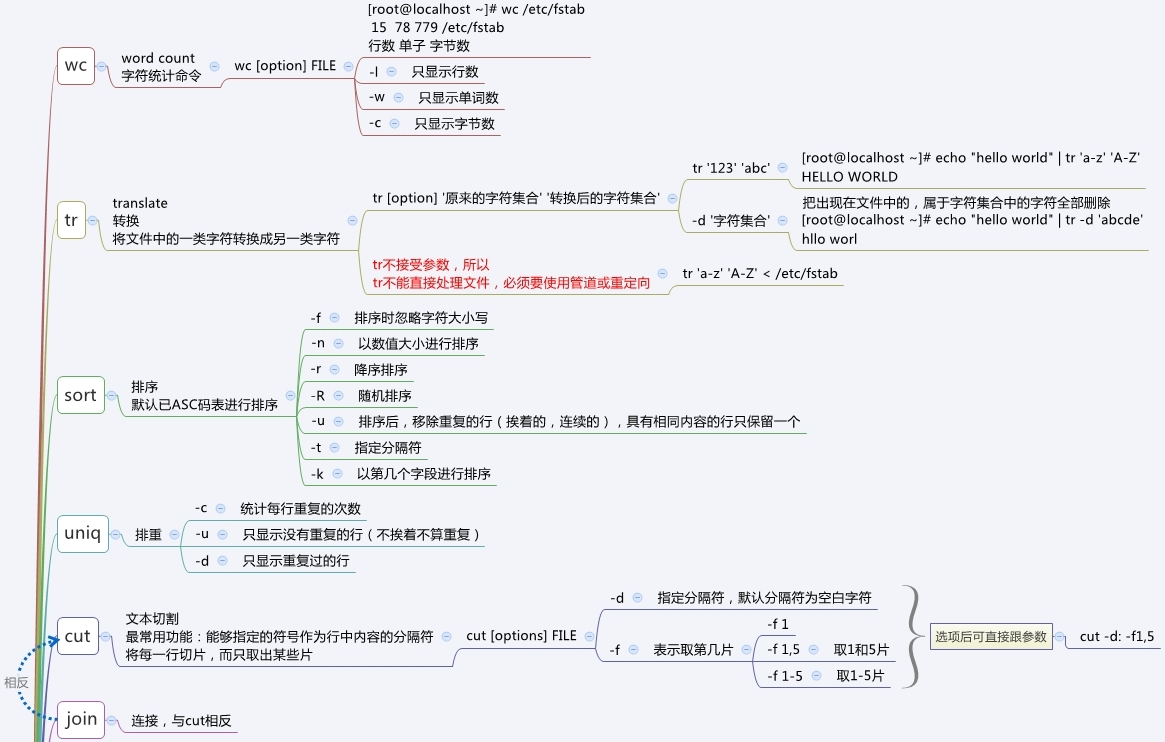
\includegraphics[width=17.5cm]{c5_text_01.jpg}\\
	  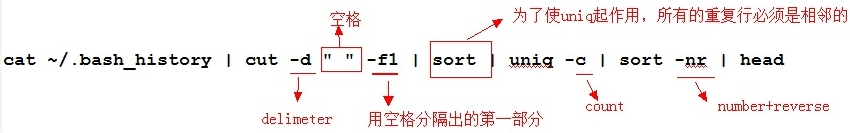
\includegraphics[width=17.5cm]{c5_text_02.jpg}\\
	  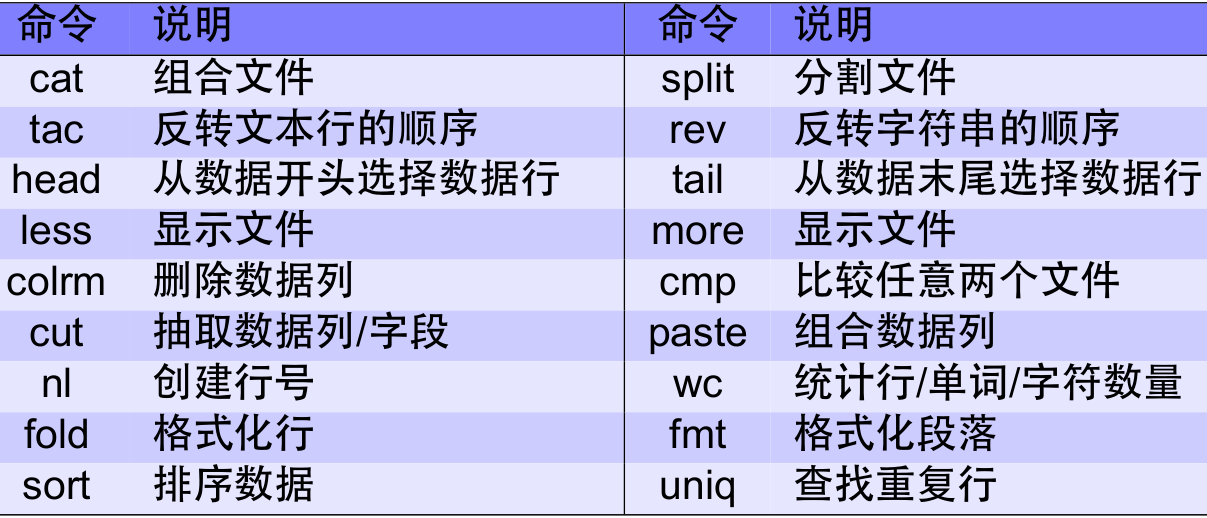
\includegraphics[width=9cm]{c5_text_03.png}
	  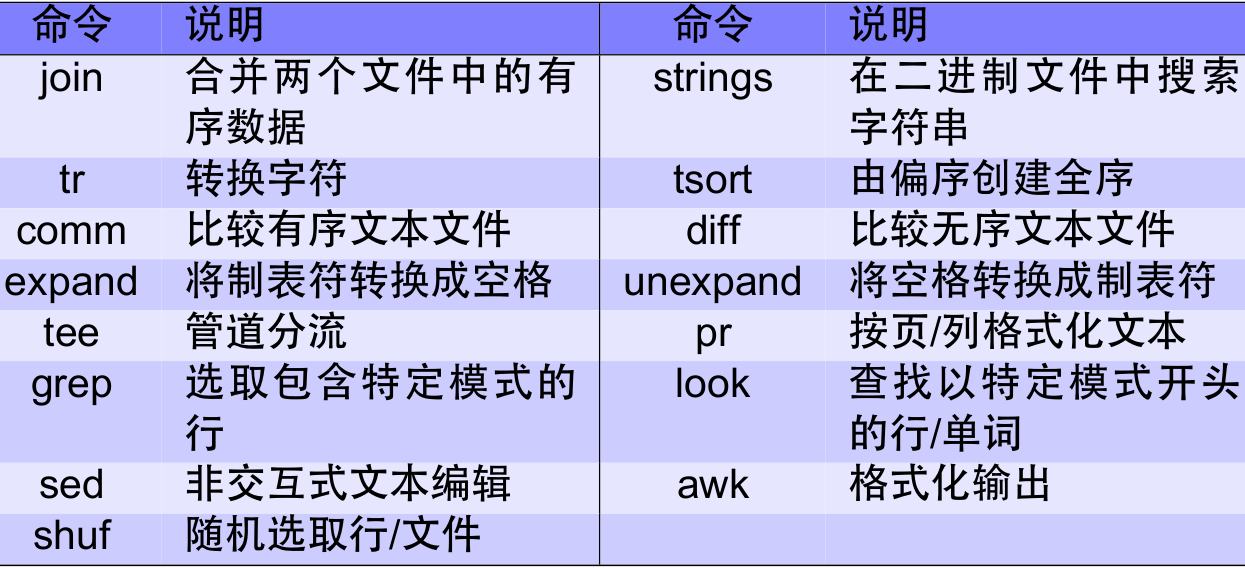
\includegraphics[width=8.5cm]{c5_text_04.png}
	\end{figure}
	\vspace*{-10pt}

  \item sed和AWK(40分钟)
    \begin{enumerate}
      \item 简介
	\begin{itemize}
\parpic[fr]{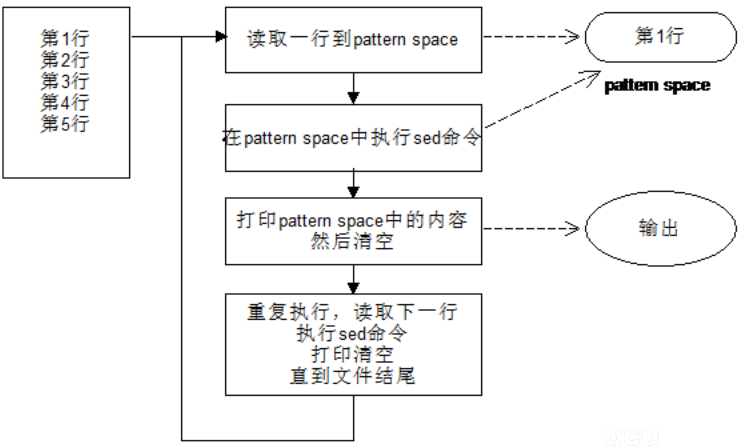
\includegraphics[width=8.5cm]{c5_sed_step_01.png}}
	  \item sed:处理纯文本流的文本编辑器
	  \item AWK:一种输出格式化语言
	  \item 对象:已有文本(管道,命令,文本文件)
	\end{itemize}
      \item \textcolor{red}{【难点】}sed\textcolor{red}{(实例讲解、操作演示)}
	\begin{enumerate}
	  \item 工作原理
	  \item 定位
	  \item 命令

\otherTail
\newpage
\otherHeader

	  \item 实例
	    \begin{itemize}
              \item \verb|sed -n '1,3!p' 123.txt|
	      \item \verb|sed -n -e '/the/p' -e '/the/=' 123.txt|
              \item \verb|sed 's/this/that/g' 123.txt|
	      \item \verb=echo "hello" | sed 's/$/.txt/g'=
              \item \verb=ls -l | sed -n '1,3p'=
	    \end{itemize}
	\vspace*{-10pt}
	\begin{figure}[h]
	  \centering
	  \hspace{1cm}
	  %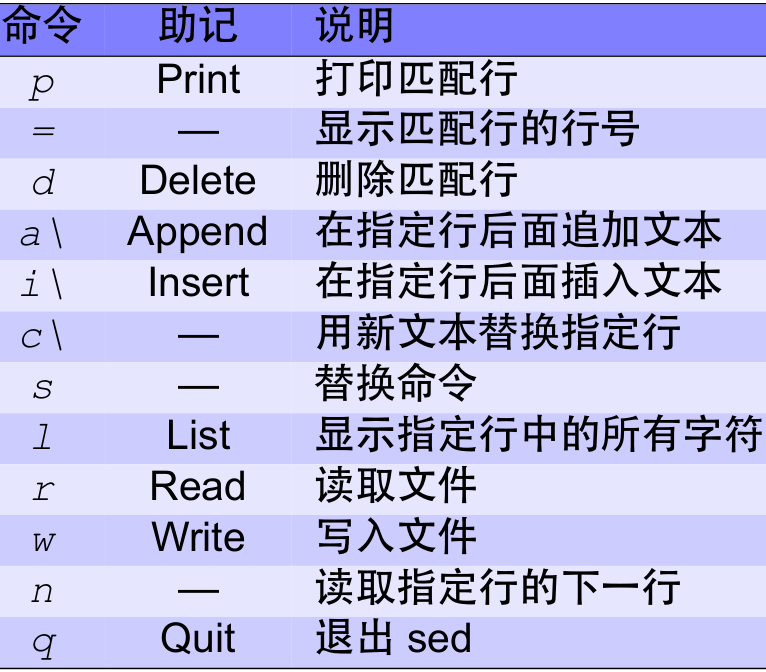
\includegraphics[width=6cm]{c5_sed_command.png}
	  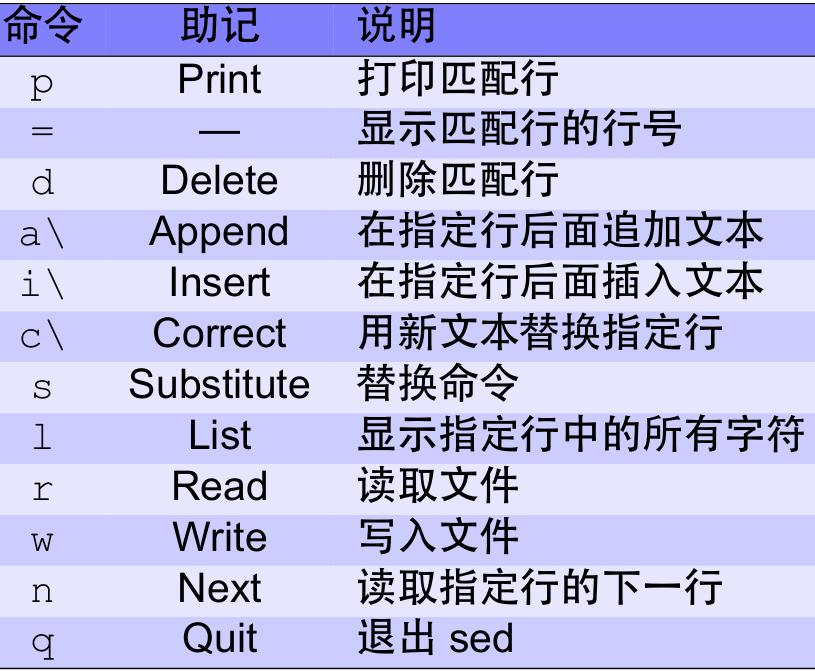
\includegraphics[width=6.5cm,height=4.5cm]{c5_sed_command_02.png}
	  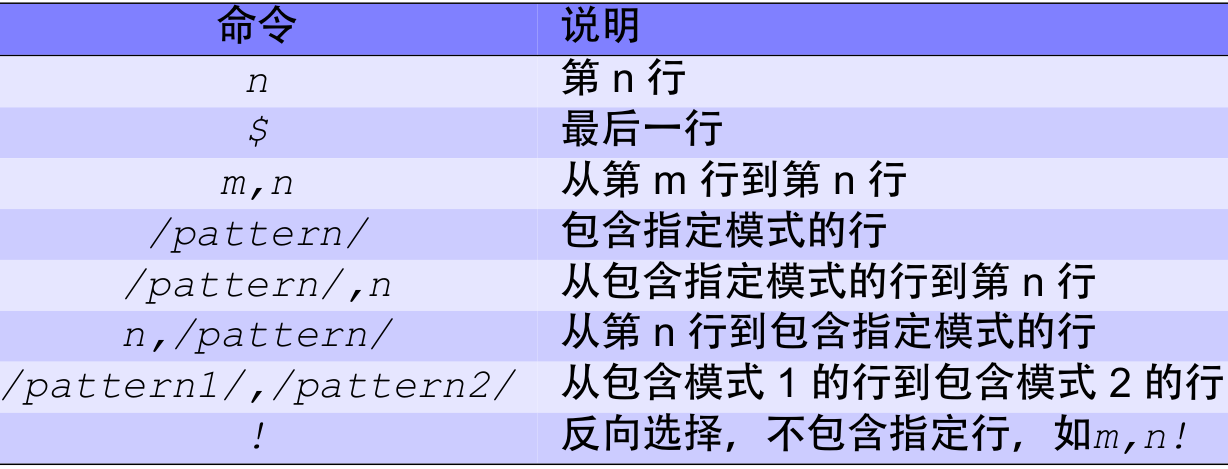
\includegraphics[width=10cm,height=4.5cm]{c5_sed_position.png}
	\end{figure}
	\vspace*{-10pt}
	\end{enumerate}


      \item \textcolor{red}{【难点】}AWK\textcolor{red}{(实例讲解、操作演示)}
	\begin{enumerate}
	  \item 工作原理
	  \vspace*{-10pt}
	    \begin{figure}[h]
	      \centering
	      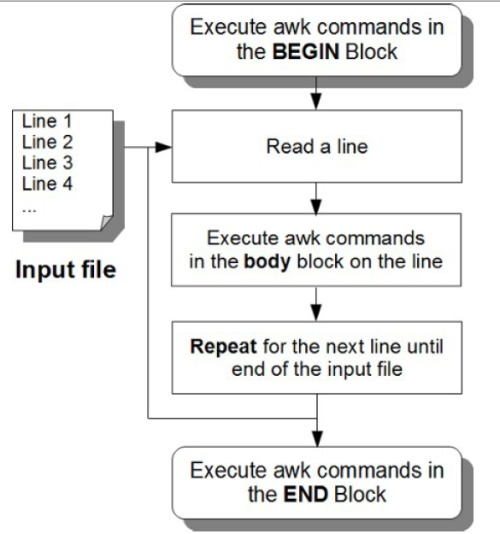
\includegraphics[width=5.3cm]{c5_awk_step_01.jpg}
	      \quad
	      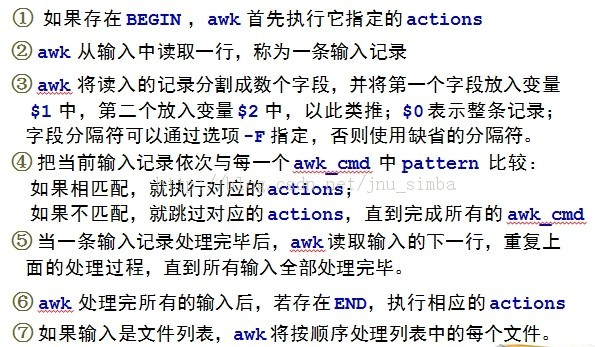
\includegraphics[width=10cm]{c5_awk_step_05.jpg}
	  \end{figure}
	  \vspace*{-10pt}
	  \item 脚本结构
	  \vspace*{-10pt}
	    \begin{figure}[h]
	      \centering
	      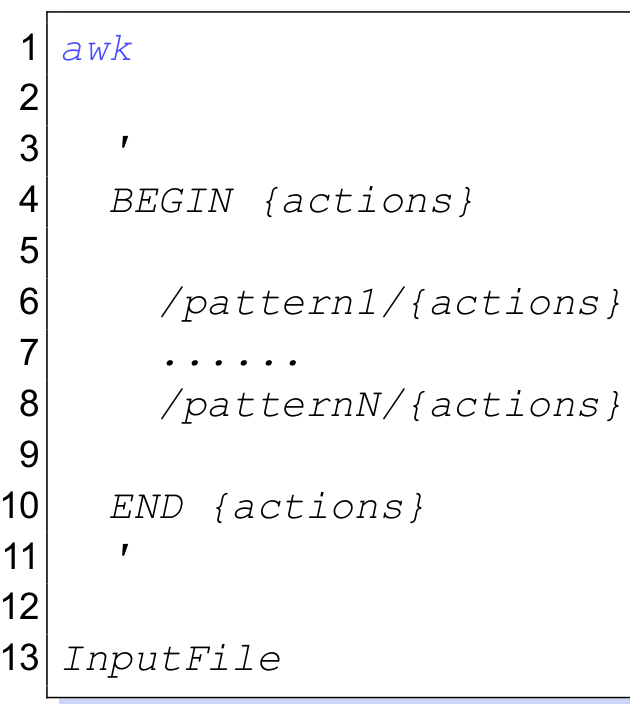
\includegraphics[width=4.5cm]{c5_awk_script.png}
	      \quad
	      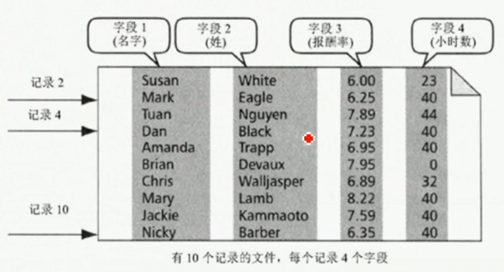
\includegraphics[width=9.3cm]{c5_awk_03.png}
	  \end{figure}
	  \vspace*{-10pt}
	  \item 常见变量
	  \item 记录与字段
	  \item 命令构成
	    \begin{itemize}
	      \item 编辑命令(一个、一组命令或一个命令文件)
	        \begin{itemize}
	          \item 模式:只编辑与模式相匹配的记录行;没有提供模式时,匹配所有行
	          \item 命令:具体执行的编辑命令;没有指定命令时,打印整个记录行
                \end{itemize}
              \item 要编辑的数据(数据或数据文件)
	    \end{itemize}

\otherTail
\newpage
\otherHeader

	  \item 实例
	    \begin{itemize}
	      \item \verb|awk '{print $0}' 123.txt|
	      \item \verb=ls -l | awk '{if($1 !~ /^d/) {print $0}}'=
	      \item \verb|awk '{printf("%03d %s\n",NR,$0)}' ori.txt > dst.txt|
	      \item \verb|awk 'BEGIN{FS=" ";OFS="\t"}{print $1,$2} ori.txt > dst.txt|
	    \end{itemize}
	  \vspace*{-10pt}
	    \begin{figure}[h]
	      \centering
	      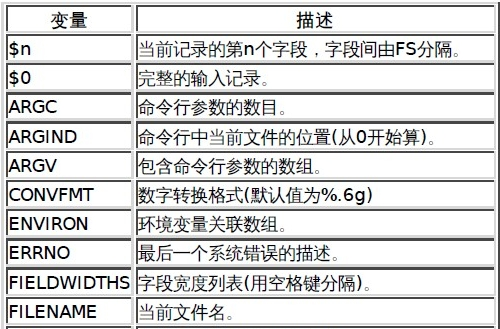
\includegraphics[width=7cm]{c5_awk_01.jpg}
	      \quad
	      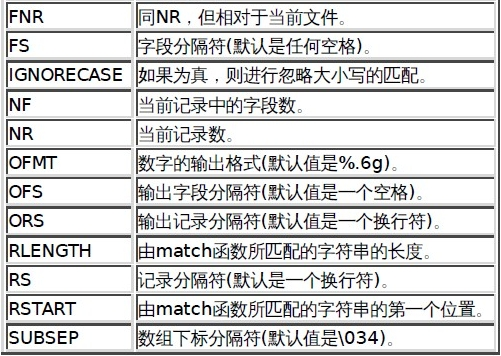
\includegraphics[width=6.5cm]{c5_awk_02.jpg}
	  \end{figure}
          \vspace*{-10pt}
	\end{enumerate}
    \end{enumerate}
  \item 生物信息学中的应用(5分钟)
    \begin{enumerate}
      \item  实例\textcolor{red}{(对命令进行逐一解析)}
	\begin{itemize}
          \item \verb=grep '>' file.fasta | wc -l=
	  \item \verb|awk '/^>/{s=++d".fa"} {print > s}' multi.fa|
          \item \verb|sed -n '1~4s/^@/>/p;2~4p' file.fq > file.fa|
          \item \verb~cat file.txt | awk '$1=="1"' |~ \\ \verb~awk '$3>=1000000' | awk '$3<=2000000'~
          \item \verb=echo {A,C,T,G}{A,C,T,G}{A,C,T,G}=
	  \item \verb|grep -c $'\tgene\t' yourannots.gff3|
          \item \verb~grep -v '^#' GFF3 | cut -s -f 3 | sort | uniq~
          \item \verb=cut -f1,6 gene.bed | sort | uniq -c | sort -nr=
          \item {\small \verb~cat myfile.fq | awk '((NR-2)%4==0){read=$1;total++;count[read]++}~ \\ \verb~END{for(read in count){if(!max||count[read]>max)~ \\ \verb~{max=count[read];maxRead=read};if(count[read]==1){unique++}};~ \\ \verb~print total,unique,unique*100/total,maxRead,count[maxRead],~ \\ \verb~count[maxRead]*100/total}'~}
	\end{itemize}
    \end{enumerate}

  \item 总结与答疑(5分钟)
    \begin{enumerate}
      \item 知识点
	\begin{itemize}
	  \item 元字符:字符,字符集,量词,边界
	  \item 正则表达式:构建,解析
	  \item find:常用测试,日常使用
	  \item grep:常用选项,日常使用
	  \item 文本处理命令:cut,wc,sort,uniq,\ldots
	  \item sed:工作原理,定位方式,编辑命令
	  \item AWK:脚本结构,工作原理,常见变量,记录,字段
	\end{itemize}
      \item 技能
	\begin{itemize}
          \item 解析并编写正则表达式
          \item find和grep的基本用法
          \item 文本处理命令的日常应用
          \item 使用sed和AWK处理文本
          \item 正则表达式在grep、sed和AWK中的应用
	\end{itemize}
    \end{enumerate}

\end{enumerate}

\otherTail


\end{document}

